\documentclass[12pt]{article}
\usepackage[margin=1in]{geometry}
\usepackage{amsmath, amsthm, amssymb, amsfonts, breqn, graphicx, subcaption}


\theoremstyle{definition}
\newtheorem{problem}{Problem}
\renewcommand*{\proofname}{Solution}
\newenvironment{custompbm}[1]
  {\renewcommand\theproblem{#1}\problem}
  {\endproblem}
\renewcommand{\theenumi}{\alph{enumi}}


\newcommand{\E}{\text{E}}
\newcommand{\V}{\text{Var}}
\newcommand{\Co}[2]{\text{Cov}\left({#1}, {#2}\right)}
\newcommand{\pdf}{\text{pdf}}
\newcommand{\pmf}{\text{pmf}}
\newcommand{\me}{\mathrm{e}}
\newcommand*\diff{\mathop{}\!\mathrm{d}}
\newcommand{\vect}[1]{\boldsymbol{#1}}
\newcommand{\mx}[1][t]{\mu_X({#1})}
\newcommand{\gx}[2]{\gamma_X({#1}, {#2})}


\title{Homework Assignment 10}
\author{Matthew Tiger}


\begin{document}


\maketitle


\begin{problem}
  Plot the energy bills versus time. What kind of trend appears to exist? What type of seasonal
  variation appears to exist? Is a transformation needed to obtain a series that displays constant
  variation?
\end{problem}

\begin{proof}
  See below for a plot of the bills time series data:
  \vskip 0mm
  \begin{center}
  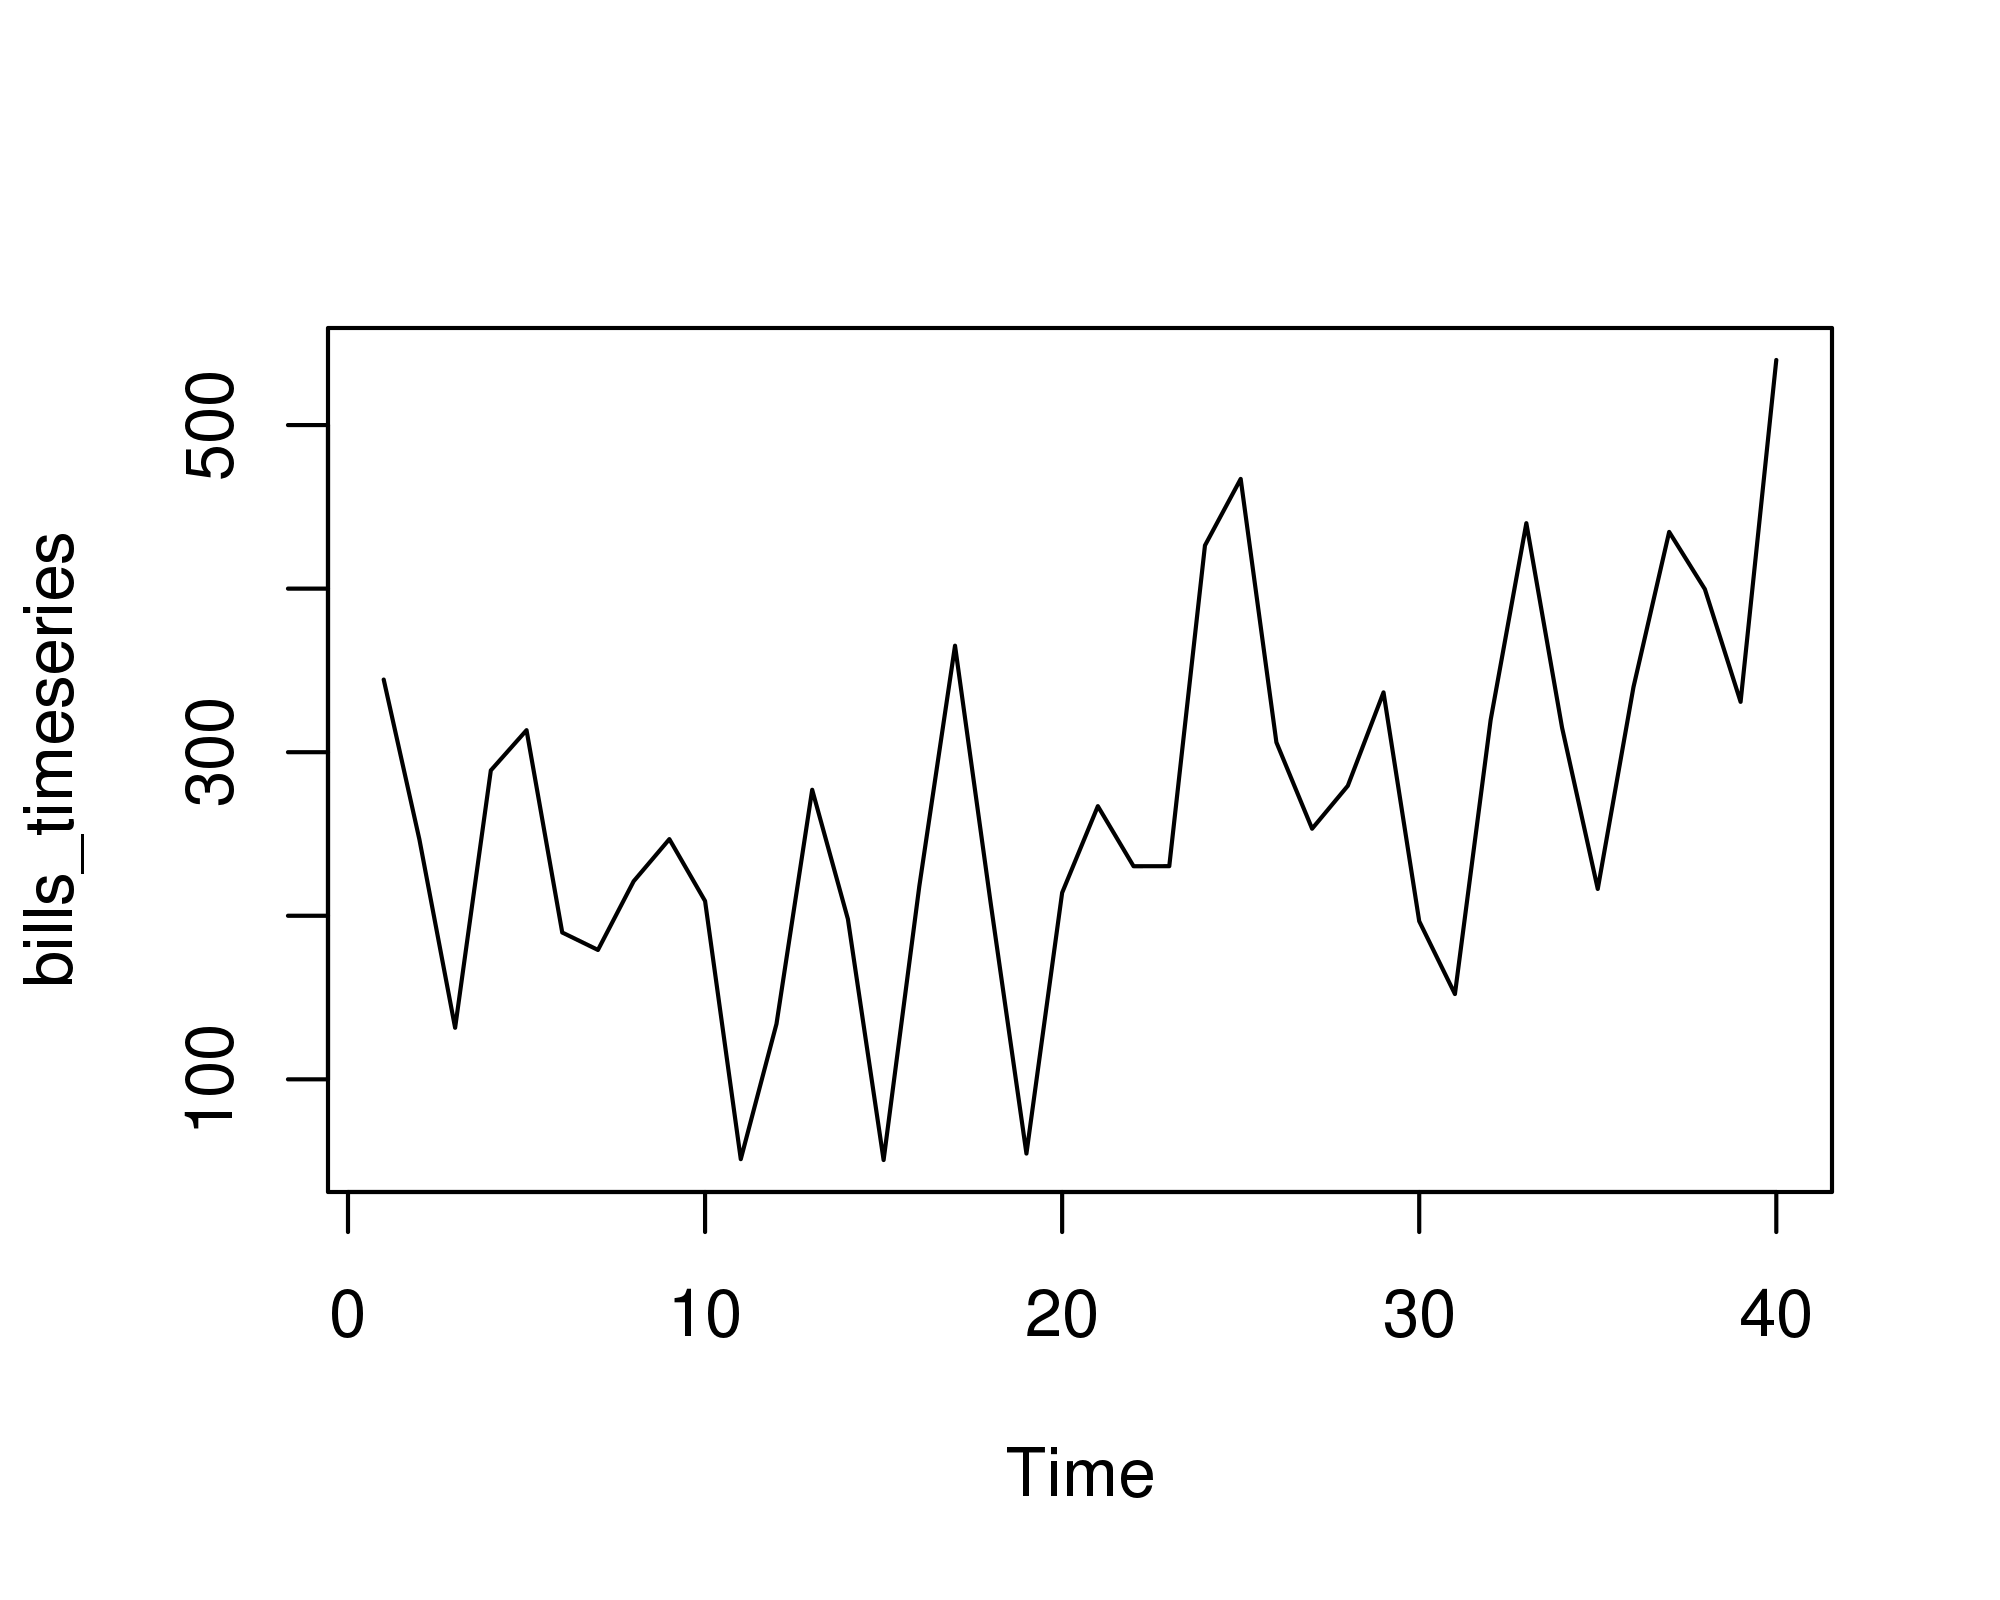
\includegraphics{timeseries}
  \end{center}
  \vskip 10mm

  It is clear from the plot that there is a trend that appears to move upwards
  as time increases and a seasonal variation with period 4
  lags present in the data so a transformation is needed to obtain residuals
  that represent a stationary time series.
\end{proof}


\begin{problem}
  Write algebraically a time series model with trend and seasonal component with definitions
  of the dummy variable.
\end{problem}

\begin{proof}
  Note that it appears that this time series has a linear trend. Additionally,
  we are interested in capturing the seasonal quarter data of the time series.
  Therefore, a time series model for the data with trend and seasonal components is given by
  \[
    X_t = a_0 + a_1 t + a_2 Q_1 + a_3 Q_2 + a_4 Q_3 + a_5 Q_4,
  \]
  where we define $Q_i$ as 1 if $t \equiv i \mod 4$ and 0 otherwise and $a_j$ is
  constant.
\end{proof}


\begin{problem}
  Are all the variables in the model statistically significant? Justify your answer.
\end{problem}

\begin{proof}
  The following \texttt{R} code performs a linear regression on our data set using the
  above equation:
  \begin{verbatim}
quarter_variable <- function(ts, position){
    vector <- rep(0, 4)
    vector[position] <- 1

    variable <- rep(vector, length(ts) / 4)

    return(variable)
}

bills <- scan("bills.csv", skip=1)
bills.ts <- ts(bills)

bills.ts.Q1 <- quarter_variable(bills.ts, 1)
bills.ts.Q2 <- quarter_variable(bills.ts, 2)
bills.ts.Q3 <- quarter_variable(bills.ts, 3)
bills.ts.Q4 <- quarter_variable(bills.ts, 4)

bills.ts.regression_equation <- bills.ts ~ 0 + time(bills.ts) +
    bills.ts.Q1 + bills.ts.Q2 + bills.ts.Q3 + bills.ts.Q4
bills.ts.regression <- lm(bills.ts.regression_equation)

# The following tells us that all variables are significant
# using a significance level of alpha = 0.05.
summary(bills.ts.regression)

  \end{verbatim}

  The code above outputs the following table displaying the significance of the
  variables in the regression equation:
  \begin{verbatim}
Coefficients:
                    Estimate Std. Error t value Pr(>|t|)
time(bills.ts)   4.8922     0.9753   5.016 1.53e-05 ***
bills.ts.Q1    256.2549    29.0803   8.812 2.08e-10 ***
bills.ts.Q2    152.0117    29.7113   5.116 1.13e-05 ***
bills.ts.Q3     62.2705    30.3606   2.051   0.0478 *
bills.ts.Q4    190.4843    31.0269   6.139 5.06e-07 ***
---
Signif. codes:  0 ‘***’ 0.001 ‘**’ 0.01 ‘*’ 0.05 ‘.’ 0.1 ‘ ’ 1
  \end{verbatim}

From this table we see that all of our of our variables are statistically significant
using a significance level of $\alpha=0.05$.
\end{proof}

\begin{problem}
  Plot the ACF and PACF of the residual. Are the residuals correlated?
\end{problem}

\begin{proof}
The following are the ACF and PACF plots of the residuals of our time series and our
regression equation.

\begin{figure}[h]
  \begin{subfigure}{.4\textwidth}
    \centering
    \includegraphics[scale=0.45]{residuals_acf}
  \end{subfigure}
  \begin{subfigure}{.7\textwidth}
    \centering
    \includegraphics[scale=0.45]{residuals_pacf}
  \end{subfigure}
\end{figure}

Note that the residuals are correlated as the ACF shows a nonzero value for a
lag greater than 0.
\end{proof}


\begin{problem}
  What is the time series model that best fits the model? Is the model statistically significant?
\end{problem}

\begin{proof}

Note that are residuals are not white noise so we need to rerun the regression
analysis using the fact that the residuals are correlated as an ARMA(1,1) model.

Rerunning the regression with this fact shows that the $Q_3$ variable is no longer
significant. Removing this variable and rerunning the analysis shows that

\begin{verbatim}
                   Value Std.Error   t-value p-value
time(bills.ts)   7.44860  1.157879  6.432974       0
bills.ts.Q1    206.68710 20.346380 10.158421       0
bills.ts.Q2     95.32084 16.141974  5.905154       0
bills.ts.Q4    130.94859 16.143011  8.111782       0

\end{verbatim}

verifying that all of our variables are now statistically significant. The ACF
of the residuals is shown below:

\begin{center}
  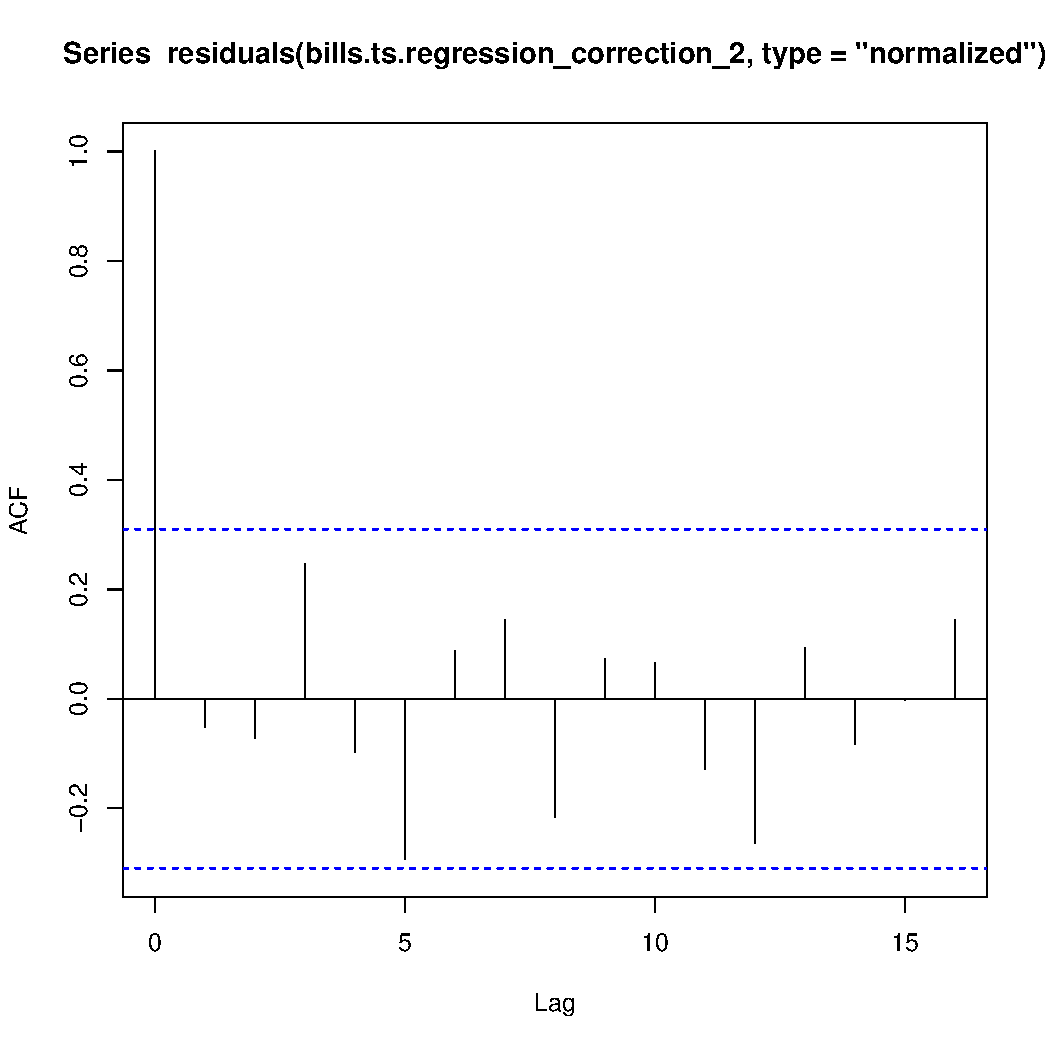
\includegraphics[scale=0.6]{new_residuals_acf}
\end{center}
From the graph, it is clear that with our new regression equation the residuals are white noise.
The underlying noise of the regression is given by the ARMA(1,1) process $\{Y_t\}$
with $Y_t = 0.6055 Y_{t-1} + Z_t + 0.3097Z_{t-1}$ with $Z_t \sim \text{WN}(0, 75.3106^2)$.

Therefore, a statistically significant time series model is given by
\[
  X_t = 7.45t + 206.68Q_1 + 95.32Q_2 + 130.95Q_4 + 0.61 Y_{t-1} + Z_t + 0.31Z_{t-1},
\]
where $Z_t \sim \text{WN}(0, 75.3106^2)$.
\end{proof}

\end{document}
